\section{Problem Definition}
\subsection{Dynamic multi-domain problem}
We clarify the Dynamic Multi-Domain Production Categorization (DMPC) problem as follows. Given a set $\mathcal{G}$ of $n$ relatively independent label taxonomies at initial time $t_0$
$$
\{G_1, G_2, G_3, ..., G_n\},
$$
each of which correlates with a domain-specific product categorization task and contains a large number of category leaf nodes respectively. The taxonomy of product categories $G_i$ is tree-structured with depth $d_i$, and it contains $m_i$ category leaf nodes:
$$
\{y_i^{(1)}, y_i^{(2)}, y_i^{(3)}, ..., y_i^{(m_i)}\} \subseteq G_i.
$$
Part of the nodes are enrolling in a dynamic trending. As time goes $t_{>0}$, the category node $y_i^{(a)}$ of a certain product might be \textbf{divided} into two categories $y_i^{(a1)}$ and $y_i^{(a2)}$ or \textbf{integrated} with another category $y_i^{(b)}$ to form $y_i^{(ab)}$. The \textbf{emergence} of a new category node $y_i^{(m+1)}$ with corresponding product title is also possible.
In addition, an emerging taxonomy $G_{n+1}$ may sprout with the new business in another domain.

A qualified system is supposed to
\begin{enumerate}
    \item jointly handle the $n$ static product taxonomy classification tasks at time $t_0$;
    \item sustain classification accuracy when the above taxonomy evolving issues are encountered;
    \item resume tolerable performance when zero-shot transfer to new taxonomy to improve cold-start user experience.
\end{enumerate}

\begin{figure*}[thbp] \centering
    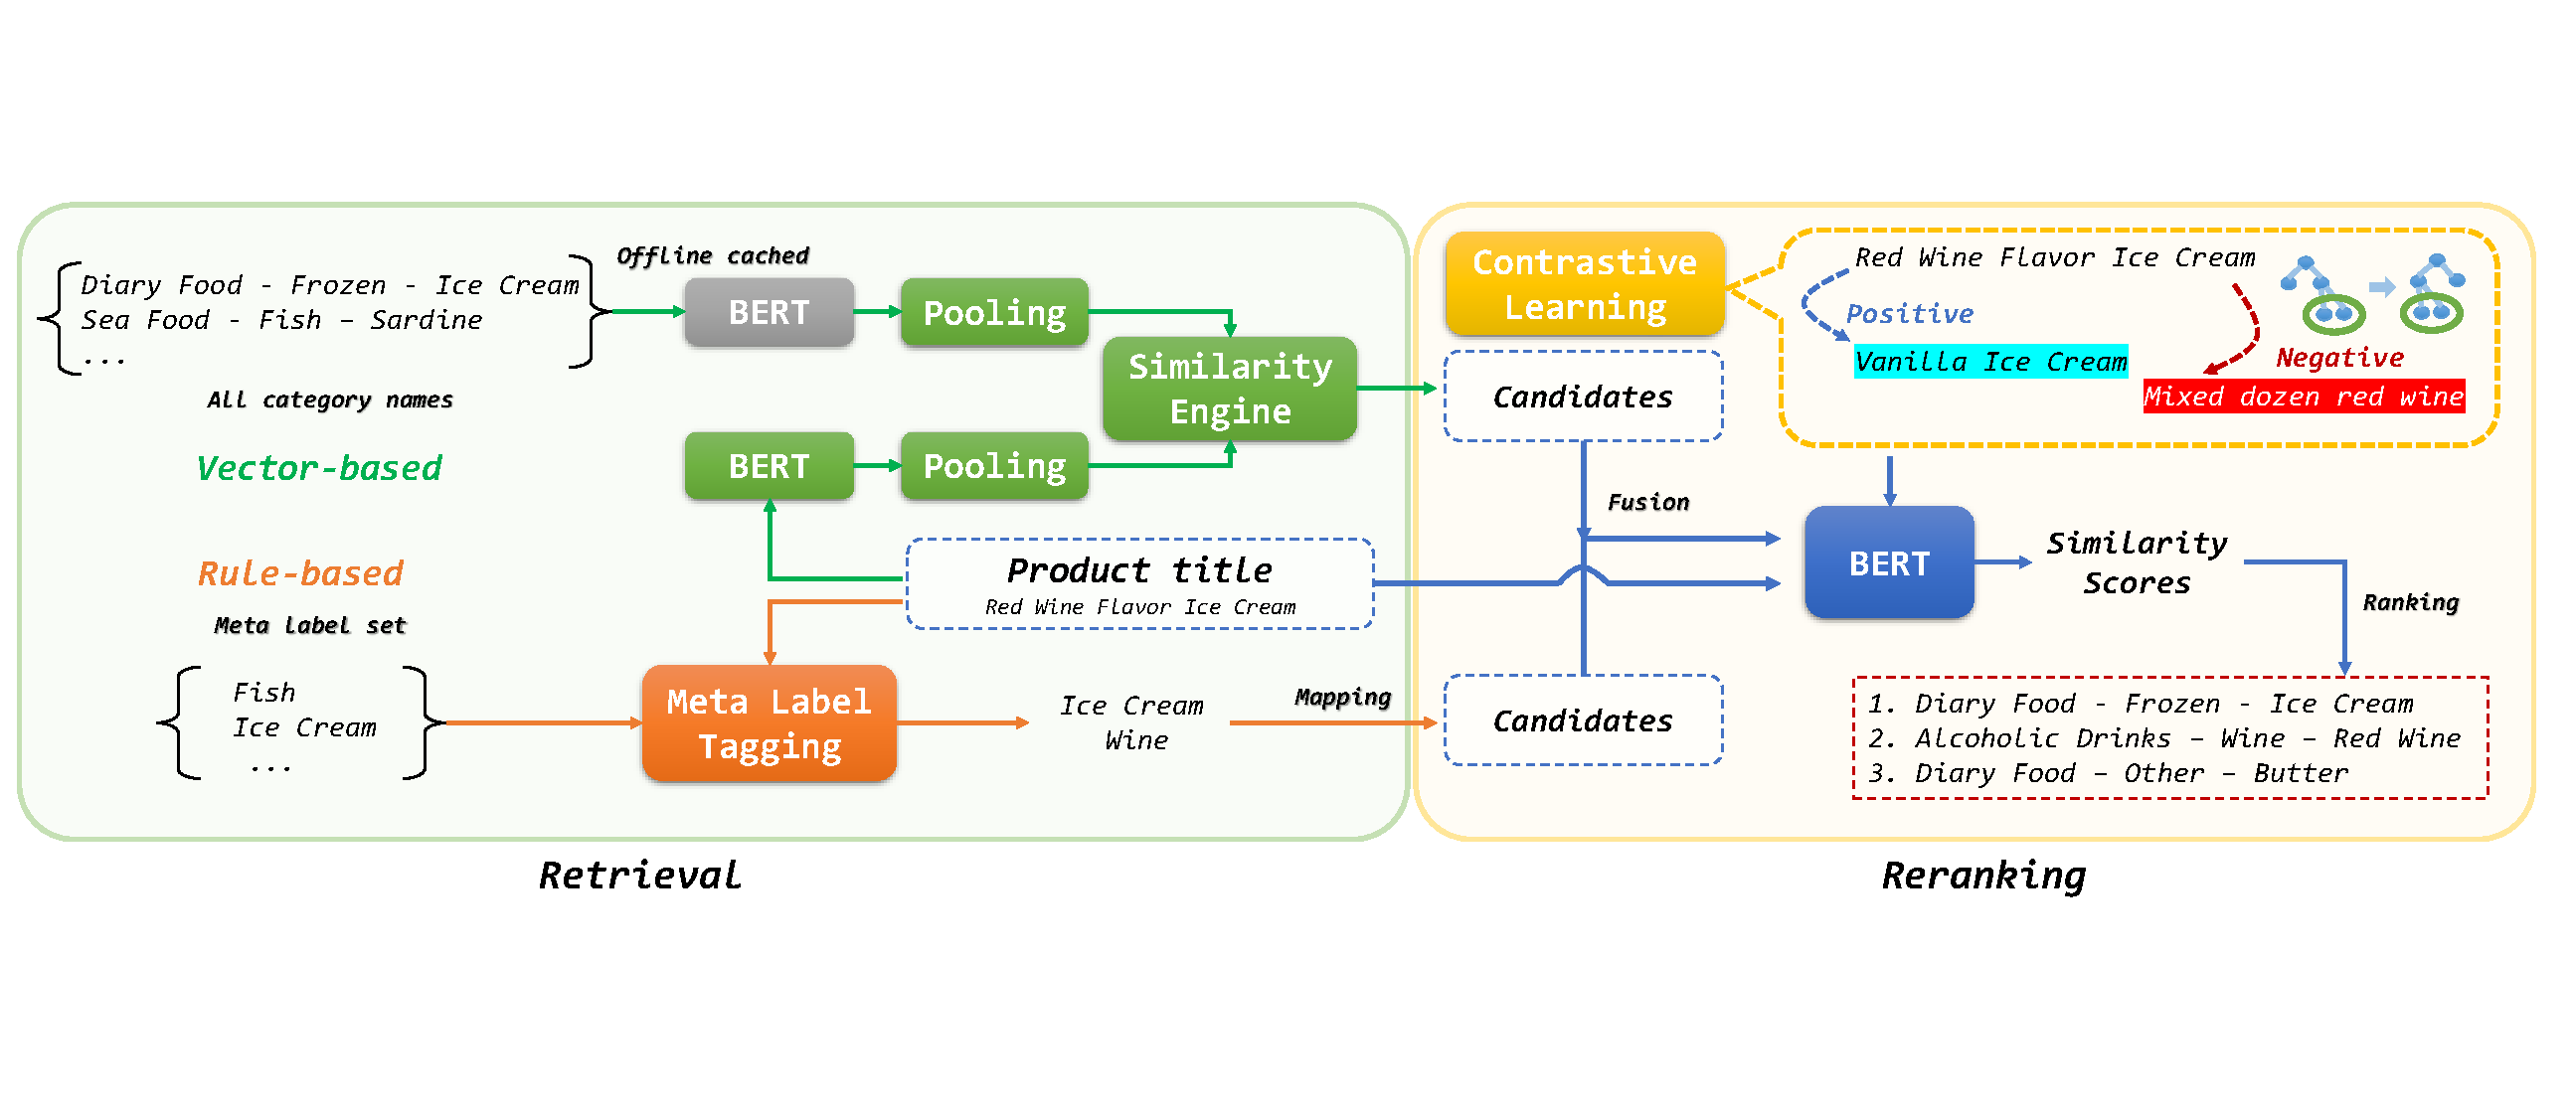
\includegraphics[width=0.99\textwidth]{pipeline5}
    \caption{An Overview of our proposed \textit{Taxonomy-agnostic Label Retrieval (TaLR)} framework. It is composed of a \textit{Retrieval} and a \textit{Reranking} stage. Our \textit{Retrieval} stage is two-fold with a vector-based unit and a rule-based unit, and two-way retrieved candidates will be tied using some heuristics. In the next \textit{Reranking} stage, generated candidates are concatenated with the product title as an input of the final scoring engine with contrastive information.} 
    \label{fig:pipeline}
\end{figure*}

\subsection{Task definition}
In previous supervised learning literature, a single product categorization task on taxonomy $G_i$ ($i=1$) is often defined as a traditional classification task, in which the training data and test data are organized in tuples 
$$
S=\{(X_i^{(1)}, y_i^{(1)}), (X_i^{(2)}, y_i^{(2)}),...,(X_i^{(m_i)}, y_i^{(m_i)}),...\}.
$$
Each $X_i$ in $S$ represents the input information of a single product and $y_i$ is the corresponding class in the taxonomy tree of labels. 

To solve DMPC problem where $i=1,2,...,n (n \geq 2)$,
in our task formulation, 
we aim to match the product title $X_i$ and the target label text $y_i$ which is the concatenation text along the path of top-bottom nodes. While previous works regard $y_i$ as meaningless label ordinals, we instead treat it equivalently with the product title as free text. 
% inspired by Sentence-Bert~\cite{reimers2019sentence}. 
Thus, the former classification task is transformed into a text semantic similarity matching and ranking task. The data samples are:
$$
S_i=\{(X_i^{(1)}, y_i^{(1)}, Y_{\mathbbm{1}}^{(1)}),...,(X_i^{(m_i)}, y_i^{(m_i)}, Y_{\mathbbm{1}}^{(m_i)}),...\},
$$
$$
S=\{S_1, S_2,...,S_i\},
$$
where $Y_{\mathbbm{1}}\in \{0, 1\}$ is an indicator label and it denotes whether the text pair $X_i$ and $y_i$ is matched ($Y_{\mathbbm{1}}=1$) or not ($Y_{\mathbbm{1}}=0$).

This reformulation is especially advantageous to simultaneously (i) capture the semantic relatedness of product titles and label texts and (ii) handle multiple taxonomies \& taxonomy evolving issues in a zero-shot manner without re-training once a unified system is well established.
% ,considering that the label text already contains rich information of this category.